\documentclass[palatino, bibnumbers]{apuntes}

\title{Geometría y Topología}
\author{Guillermo Julián Moreno}
\date{15/16 C2}

% Paquetes adicionales
\usepackage{enumitem}
\usepackage{tikztools}
\usepackage{fancysprefs}
\usepackage{tikz-3dplot}
\usepackage{xfrac}
\usepackage{wrapfig}
\usepackage{fastbuild}

\usetikzlibrary{arrows}
\usetikzlibrary{patterns}
\usetikzlibrary{intersections}
\usetikzlibrary{calc}
\usetikzlibrary{fadings}

\setlist{itemsep=1pt, topsep=5pt}
\bibliographystyle{alpha}
% --------------------

\precompileTikz

\newcommand{\Id}{\mop{Id}}
\newcommand{\cln}{\colon\!}

\begin{document}
\pagestyle{plain}

% http://tex.stackexchange.com/a/14243
\relpenalty=9999
\binoppenalty=9999

\begin{abstract}
Estos son los apuntes del curso de Geometría y Topología, del profesor Gabino González.
\end{abstract}

\maketitle


\tableofcontents
\newpage
% Contenido.

\chapter{Conceptos básicos - Variedades}

En Geometría, los objetos que estudiamos se llaman ``variedades''. Veremos de distintos tipos (por ejemplo, en Geometría Diferencial \citep{ApuntesGeoDif} veíamos variedades diferenciables), aunque nosotros empezaremos con las topológicas.

\begin{defn}[Variedad\IS topológica] Una variedad topológica es un espacio topológico $M$ con las siguientes propiedades:
\begin{enumerate}
\item $M$ es $T_2$ (esto es, \concept{Hausdorff}: dos puntos distintos tienen entornos disjuntos).
\item $∀p ∈ M$ admite un entorno $U$ y un homeomorfismo $\appl{φ_u}{U}{ℝ^N}$ (o $\bola^N$).

Al par $(U,φ_u)$ se le llama \concept{Carta} para $p$. Si $φ_u(p) = 0$, se dice que la carta está centrada en $p$. A la colección de cartas se le llamará \concept{Atlas}.
\item Si para cualquier par de cartas $(U,φ_u)$ y $(V,φ_v)$ la aplicación $$\appl{φ_v ○ \inv{φ_u}}{φ_u(U∩V)}{φ_v(U∩V)}$$ es difeomorfismo, estamos entonces ante una \concept{Variedad\IS diferenciable}.
\end{enumerate}
\end{defn}

\begin{figure}[thbp]
\centering
\inputtikz{Cartas}
\caption{Un esquema de las cartas de una variedad $M$ y cómo se comportan en la intersección.}
\label{fig:Cartas}
\end{figure}

La dimensión de la variedad está dada por la dimensión de $ℝ$ a la que son homeomorfas las cartas. La cuestión es que no tenemos claro si eso está bien definido. En el caso diferenciable, la condición de difeomorfismo para la intersección de cartas implica que la dimensión de ambas cartas ha de ser la misma. En el caso topológico también está bien definido, aunque es más difícil de demostrar ya que dependemos de que no exista un homeomorfismo entre $ℝ^n$ y $ℝ^m$ con $n ≠ m$, que no es trivial.

Un ejemplo sencillo de variedad es $M = \bola^N$, con $φ$ la identidad. Otro ejemplo es $\crc$ (la circunferencia), que es una variedad de dimensión 1, que no se puede dar con sólo una carta (la circunferencia no es homeomorfa a $ℝ$)\footnote{$\crc$ es compacta y $\real$ no, y como compacidad es propiedad topológica y los homeomorfismos las preservan, no pueden ser homeomorfas.}. Podríamos darla tomando las dos mitades superior e inferior usando senos y cosenos, y también podríamos hacer la proyección estereográfica (\ref{fig:ProyEstereo}) desde los polos norte y sur $(0,1), (0,-1)$ respectivamente sobre la recta real. En este caso, tendríamos las siguientes cartas: \[
\begin{matrix}
	\appl{α_1}{V_1 = \crc\setminus\set{(0,1)}&}{&ℝ} \\
	p=(s,t) &\longmapsto& \frac{s}{1-t}
\end{matrix}
\qquad
\begin{matrix}
	\appl{α_1}{V_2 = \crc\setminus\set{(0,-1)}&}{&ℝ} \\
	p=(s,t) &\longmapsto& \frac{s}{1+t}
\end{matrix}\]

\begin{figure}[hbtp]
\inputtikz{ProyeccionCirc}
\caption{Proyección estereográfica de la circunferencia.}
\label{fig:ProyEstereo}
\end{figure}

Para comprobar si este atlas es diferenciable, tendríamos que mirar qué ocurre con $α_2 ○ \inv{α_1}$. Después de un montón de cuentas\footnote{Ver \fref{sec:proyeccion_estereografica_crc}.}, nos sale que efectivamente lo es ($α_2 ○ \inv{α_1} = \frac{1}{x}$) en el dominio en el que está definido (el cero no es un problema porque no está dentro del dominio).

Trivialmente, podemos definir cuándo dos atlas son compatibles.

\begin{defn}[Atlas\IS compatibles] Se dice que dos atlas $A_1, A_2$ son compatibles si $A_1 ∪ A_2$ es un atlas. Esto es, si y sólo si las cartas de $A_1$ son compatibles con las de $A_2$.
\end{defn}

Por ejemplo, podemos estudiar si los dos atlas que hemos visto para la circunferencia \crc son compatibles (recordamos que uno era el trigonométrico y otro la proyección estereográfica). Esto es equivalente a preguntarnos si $α_j ○ \inv{φ_i}$ son diferenciables. Se puede ver fácilmente que \[ α_1 ○ \inv{φ_1} (θ) = α_1(\cos θ, \sin θ) = \frac{\cos θ}{1 - \sin θ}\] que es diferenciable. Así podríamos hacerlo con el resto de combinaciones, y por lo tanto tenemos que ambos atlas dan la misma variedad.

Como ejercicio, podríamos dar un atlas $A_3$ en \crc con cartas en forma de semicircunferencia y después comprobar que es compatible con los dos atlas de antes. Otro ejercicio más largo sería hacer lo análogo para $\crc[2]$.

Una vez que tenemos ya definido qué es una variedad, el siguiente paso es saber si podemos hacer análisis ahí: si podemos definir aplicaciones diferenciables en ella o si podemos integrar una función. La segunda parte la veremos más adelante con las formas diferenciales, pero la primera la podemos estudiar ahora.

\begin{figure}[hbtp]
\centering
\inputtikz{ApplDiferenciable}
\caption{Esquema de la definición de la aplicación diferenciable entre dos variedades en base a las cartas.}
\label{fig:ApplDiferenciable}
\end{figure}

\begin{defn}[Aplicación\IS diferenciable] Una aplicación continua $\appl{f}{M}{N}$ entre dos variedades $M$ y $N$ es diferenciable si $∀p ∈ M$ con $f(p) = q ∈ N$ existe una carta $(U,φ_U)$ alrededor de $p$ y una carta $(V, φ_V)$ alrededor de $q$ tal que $f(U) ⊂ V$ y $\appl{φ_V○f ○ \inv{φ_U}}{\bola^m}{\bola^n}$ es diferenciable.
\end{defn}

Es importante ver que este concepto de diferenciabilidad no depende de las cartas elegidas para cada punto. Suponiendo que tenemos otras dos cartas $α_U, α_V$ alrededor de $p$ y $q$ tendríamos que \[ α_V ○ f ○ \inv{α_U} = (α_V ○\inv{φ_V}) ○ (φ_V ○ f ○ \inv{φ_U}) ○ (φ_U ○ \inv{α_U})\]

Por compatibilidad de las cartas, $α_V○\inv{φ_V}$ y $φ_U ○ \inv{α_U}$ son diferenciables. Además, ya que hemos dicho que $f$ es diferenciable con las cartas $φ_U, φ_V$ luego $φ_V ○ f ○ \inv{φ_U}$ es diferenciable igualmente. Así, la composición de esas tres funciones es diferenciable.

\begin{example} Vamos a definir una función entre variedades y ver si es diferenciable. No nos complicaremos mucho: \begin{align*}
\appl{f}{\crc&}{\crc ⊂ ℂ} \\
z &\longmapsto \conj{z}
\end{align*}

Haciendo los cálculos, vemos que \[ φ_1 ○ f ○ \inv{φ_1} (θ) = φ_1 ○ f(e^{iθ}) = φ_1(e^{-iθ}) = \begin{cases} -θ \\ -θ + 2θ \end{cases} \] que efectivamente es diferenciable.
\end{example}


\begin{example} Definimos ahora una función a priori menos interesante, la identidad: \begin{align*}
\appl{f}{M&}{N} \\
p &\longmapsto p
\end{align*}

$M$ será $(ℝ,φ)$ y $N = (ℝ,α)$, con $φ$ la identidad y $α(t) = t^3$. Es obvio ver que $f$ es diferenciable (si hacemos la composición nos sale directamente). Ahora bien, si tomamos $\appl{f}{N}{M}$, ¿sigue siendo diferenciable? En este caso, si calculamos vemos que $φ ○ f ○ \inv{α}(t) = \sqrt[3]{t}$ pero esta aplicación no es diferenciable en $0$. Esto es lo mismo que decir que estos dos atlas en $ℝ$ no son compatibles: no definen la misma estructura. Sí serían compatibles si estuviésemos hablando sólo de variedades topológicas, porque sí que estamos ante un homomorfismo.
\end{example}

Una vez que hemos visto qué es una variedad, podemos ver cómo construir variedades combinándolas de distintas maneras.

\section{Variedades producto}

La primera opción para construir una variedad es el producto cartesiano, que ya conocemos de otro tipo de conjuntos.

\begin{defn}[Variedad\IS producto] Sean $M^m$, $N^n$ variedades con sus respectivos atlas $A_1 = \set{(U_i, φ_i)}_{i ∈ I}$ y $A_2 = \set{(V_i, α_j)}_{j ∈ J}$. Entonces, la variedad producto es $M×N^{m+n}$ con atlas \[ A_1 × A_2 = \set{(U_i×V_j, φ_i × α_j)}_{(i,j) ∈ I × J} \]
\end{defn}

Un ejemplo sencillo es $\crc × ℝ$, una variedad con cartas de la forma $(φ_1 × α_1) = ((x,y), t)$, donde $(x,y)$ vienen de la carta de la circunferencia que hayamos escogido. En este caso, la variedad es $M = \set{(x,y,z) \tq x^2 + y^2 = 1}$, el cilindro, ya que podemos tomar $\appl{f}{M}{\crc × ℝ}$ es un difeomorfismo (se pueden hacer las cuentas pero son triviales).

Otro es $\crc × \crc$, que nos podemos preguntar si es difeomorfa a $\crc[2]$, más que nada porque uno es un toro y otro una esfera. Sin embargo, un argumento más formal implicaría usar los grupos fundamentales\footnote{Ver \citep[Cap. III]{ApuntesTopologia}.}, ya que $π(\crc[2]) = \set{0}$, $π(\crc) = ℤ$ y por lo tanto $π(\crc × \crc) \simeq ℤ × ℤ$. Los grupos fundamentales no son isomorfos por lo que no puede haber difeomorfismo. Lo malo es que este argumento no nos vale para decir, por ejemplo, si $\crc[2] × \crc[3] \simeq \crc[5]$. En realidad, no sin siquiera homeomorfas, pero para saberlo tendremos que usar las cohomologías de De Rham (\fref{chap:CohomologiaDeRham}).

Durante el curso, veremos más herramientas para saber si existen o no difeomorfismos entre variedades.

\section{Variedad cociente}

En las variedades también se puede aplicar el análogo del conjunto cociente. Eso sí, necesitaremos ciertas condiciones ``extra'' sobre la variedad.

\begin{defn}[Variedad\IS cociente] Sea $M$ una variedad y sea $G < \mop{Diff}(M)$ un subgrupo de los difeomorfismos sobre $M$, tal que $\abs{G} < ∞$ y además $G$ actúa libremente en $M$ (esto es, que $∀g ∈ G$ distinta de la identidad y $∀x ∈ M$ se tiene que $g(x) ≠ x$).

Entonces, definimos el espacio cociente $\quot{M}{G}$ a través de la relación de equivalencia \[ x \sim y \iff ∃g ∈ G \tq  y = g(x) \]

La estructura de variedad se la damos considerando la proyección canónica \begin{align*}
\appl{π}{M&}{\quot{M}{G}} \\
x &\longmapsto [x]
\end{align*} que a cada elemento le asigna su clase.
\end{defn}

Por ejemplo, si consideramos la variedad $M = \crc[2]$ y el grupo $G = \gen{J} = \set{\Id, J}$ con $J(x,y,z) = (-x,-y,-z)$. En este caso, $\projp^2 = \quot{\crc[2]}{\gen{J}}$.

\begin{figure}[hbtp]
\centering
\inputtikz{EsferaPlanoProj}
\caption{Paso de la esfera al plano proyectivo, con la proyección canónica π.}
\label{fig:EsferaPlanoProj}
\end{figure}

Para darle la estructura de atlas, tomamos una carta $(U,φ_U)$ en $M$ tal que $U ∩ g(U) = \set{∅}\;∀g ∈ G$, por lo que $\appl{\restr{π}{U}}{U}{\quot{M}{G}}$ es un homeomorfismo sobre su imagen $π(U)$, luego biyectivo. Así, las cartas en $\quot{M}{G}$ son de la forma $\left(π(U), φ_U ○ \inv{\restr{π}{U}}\right)$.

En este caso, nos podemos preguntar qué ocurre si $π(U) ∩ π(V) ≠ ∅$ para dos cartas $U,V$: ¿es $\left(φ_V ○ \inv{\restr{π}{V}}\right) ○ \left(\restr{π}{U} ○ \inv{φ_U} \right)$ diferenciable?

La cuestión es que $\inv{\restr{π}{V}} ○ \restr{π}{U} = g ∈ G$ por la construcción de $g$\footnote{Si $π(x) = π(y)$, son de la misma clase y por lo tanto hay un difeomorfismo que lleva de $x$ a $y$.}, y por lo tanto nos queda que $φ_V ○  g ○ \inv{φ_U}$ es diferenciable así que la estructura de atlas que nos queda es compatible.

Un ejemplo muy común es $\projp^n = \quot{\crc[n]}{\gen{J}}$ para $n ∈ ℕ$, que son los espacios proyectivos reales de dimensión $n$.

Esta teoría también funciona siempre que el grupo $G$ cumpla la segunda propiedad y además $∀x ∈ M$ exista un $U$ tal que $g(U) ∩ U = ∅$ $∀g ≠ \Id$.

Otros ejemplos son $\quot{ℝ}{ℤ} \simeq \crc$ o $\quot{ℝ^2}{ℤ^2} \simeq \crc × \crc$. Ambos son análogos: el primero lleva a la circunferencia y el segundo al toro. Es fácil de ver aunque hay que echarle un poco de imaginación: lo vamos a desarrollar con $\quot{ℝ^2}{ℤ^2}$. En este caso, consideramos $ℤ^2$ como el conjunto de los difeomorfismos en $ℝ^2$ de la forma $f(x,y) = (x+m, y+n)$ con $(m,n) ∈ ℤ^2$, que es obviamente un grupo que no fija puntos. En este caso, el hecho de que sea infinito no nos causa demasiados problemas.

\begin{figure}[hbtp]
\centering
\inputtikz{ToroEspacioCociente}
\caption{Un gráfico para mostrar cómo $\protect\quot{ℝ^2}{ℤ^2}$ es homeomorfo a un toro: la proyección canónica $π$ nos lleva al cuadrado $[0,1]×[0,1]$ con los bordes conectados (los del mismo color). Si pudiésemos ``moldear'' el cuadrado y pegar los bordes, estaríamos ante el toro.}
\label{fig:ToroEspacioCociente}
\end{figure}

La relación de equivalencia que usamos para construir el espacio cociente nos dice que dos puntos $x,y ∈ ℝ^2$ pertenecen a la misma clase si existe un difeomorfismo $g ∈ ℤ^2$ tal que $g(x) = y$. En otras palabras, si tenemos un par $(m,n) ∈ ℤ^2$ tal que $(x_1 + m, x_2 + n) = (y_1, y_2)$, entonces $x = (x_1, x_2)$ y $y=(y_1, y_2)$ están relacionados, por lo que nuestro conjunto de clases de equivalencia son los puntos en $[0,1] × [0,1]$. Eso sí, con una peculiaridad: los bordes están ``unidos'', el de arriba con el de abajo y el de la izquierda con el de la derecha. Es decir, que topológicamente estamos ante un toro (ver \fref{fig:ToroEspacioCociente}).

Si por otra parte trabajásemos con $\quot{ℝ}{ℤ}$, tendríamos algo similar: estaríamos identificando los dos bordes del intervalo $(0,1)$ y tendríamos una circunferencia. Para demostrarlo formalmente, tendríamos que definir una aplicación \begin{align*}
\appl{f}{\quot{ℝ}{ℤ}&}{\crc} \\
[x] &\longmapsto e^{2πix} = (\cos 2πx, \sin 2πx)
\end{align*} y comprobar que es diferenciable, esto es, tenemos que comprobar que $\inv{φ_U} ○ f ○ α$ es diferenciable, teniendo que $φ_U$ es una carta de $\quot{ℝ}{ℤ}$, con $\inv{φ_U} = \restr{π}{U}$ la proyección canónica restringida a $U$; y $α(e^{2πiθ}) = 2πθ$ la otra carta. La composición sería obviamente $π ○ f ○ α = 2πx$ que es diferenciable.

Otro ejemplo posible es ver si podemos definir un difeomorfismo entre $\projp^1$ y $\crc$ como $ρ(z) = z^2$, con $z ∈ ℂ$. Eso sí, sólo pasa con $n=1$: en general, $\projp^n \nsim \crc[n]$.

\subsection{Espacios proyectivos}

A través de la variedad cociente hemos hablado de espacios proyectivos. Vamos a definirlos bien:

\begin{defn}[Espacio\IS proyectivo] Sea \kbb un cuerpo\footnote{En nuestro caso, $ℝ$ o $ℂ$}. Entonces definimos el plano proyectivo como \[ \mathbb{P}^n(\kbb) = \quot{\kbb^{n+1} \setminus \set{0}}{\sim}\] con $\sim$ la relación de equivalencia dada por $x \sim y \iff y = λx$ para algún $λ ∈ \kbb^*$.
\end{defn}

Cuando \kbb es $ℝ$ o $ℂ$, $\mathbb{P}^n(\kbb)$ es una variedad de dimensión $n$ o $2n$ respectivamente.

Las cartas en el plano proyectivo son de la forma\footnote{Como notación, los dos puntos denotan clases de equivalencia, esto es, $[x_1\cln x_2] \equiv \set{\gor{x_1}, \gor{x_2}}$.} \[ U_k = \set{[x_1\cln x_2\cln \dotsb\cln x_k\cln \dotsb\cln x_n] ∈ \mathbb{P}^n(\kbb) \tq x_k ≠ 0} \]

Este conjunto está bien definido. No lo estaría si estuviésemos diciendo que $x_k = 1$, por ejemplo, porque tendríamos que $[1\cln 1\cln 1] = [3\cln 3\cln 3]$ y no quedaría claro si está o no en el conjunto.

Además, se ve fácilmente que $\bigcup_{k=0}^n U_k = \mathbb{P}^n(\kbb)$. Sólo nos queda definir una biyección \begin{align*}
\appl{φ_k}{U_k&}{\kbb^n} \\
[x_1\cln \dotsb\cln x_k\cln \dotsb\cln x_n] &\longmapsto \left(\frac{x_0}{x_k}, \dotsc, \frac{x_n}{x_k}\right)
\end{align*}

La inversa de $φ_k$ sería \[ \inv{φ_k}(y_1, \dotsc,y_n) = [y_1\cln \dotsb \cln y_{k-1} \cln 1 \cln y_{k+1}\cln \dotsb \cln y_n]\]

Sólo nos queda comprobar que las funciones transición $\appl{φ_j ○ \inv{φ_k}}{\kbb^n \setminus \set{y_j = 0}}{\kbb^n \setminus \set{y_k = 0}}$ son diferenciables. Vemos que \[ (φ_j ○ \inv{φ_k})(y_1, \dotsc, y_n) = φ_j\left([y_1\cln \dotsb \cln y_{k-1} \cln 1 \cln y_{k+1}\cln \dotsb \cln y_n]\right) = \left(\frac{y_1}{y_j}, \dotsc, \frac{1}{y_j}, \dotsc, \frac{y_n}{y_j} \right)\], que efectivamente es diferenciable porque en el espacio de partida $y_j ≠ 1$.

Así, tenemos que tanto $\mathbb{P}^n(ℝ) = \projp^n$ y $\mathbb{P}^n(ℂ) = \projcp^n$ son variedades diferenciables.

El plano proyectivo complejo es interesante. Por ejemplo, podemos ver que $\projcp^1 \simeq ℂ^2 ∪ \set{∞} \simeq \crc[2]$. Otro aspecto interesante de $\projcp^n$ es que no sólo es diferenciable como comentábamos antes: también es holomorfa. Y lo relevante de las variedades holomorfas es que son todas orientables. Esto nos sirve como excusa para introducir otro tipo de variedades.

\section{Variedades orientables}

\begin{defn}[Variedad\IS orientable] \label{def:VariedadOrientable} Una variedad $M$ es orientable si existe un atlas $A = \set{(U_i,φ_i)}_{i∈I}$ tal que $\abs{\Dif (φ_j○\inv{φ_i})} > 0$ para cualesquiera $j,i ∈ I$.
\end{defn}

Un atlas holomorfo siempre verificará la condición de orientabilidad por las ecuaciones de Cauchy-Riemann \citep[Sección III.2]{ApuntesVarCompI}. Definiendo $\appl{f = (φ_j○\inv{φ_i})}{ℂ}{ℂ}$ holomorfa, tenemos que $f = u + iv$ y entonces \[ \Dif f = \det \begin{pmatrix}
u_x & u_y \\ v_x & v_y
\end{pmatrix} \eqreasonup{Eq. CR} \det
\begin{pmatrix}
u_x & -v_x \\ v_x & u_x \end{pmatrix} = u_x^2 + v_x^2 > 0 \]

Otro ejemplo interesante es $\quot{ℝ×(-a,a)}{ℤ}$, de tal forma que $n·(x,λ) = (x+n,λ)$. Es un cilindro (identificamos los dos lados de un rectángulo de anchura infinita y altura $2a$) y orientable.

\begin{wrapfigure}{r}{0.4\textwidth}
\centering
\begin{tikzpicture}
\fill[blue!20!white] (0, -0.8) rectangle (2, 0.8);
\draw (-1,0) -- (3,0);
\draw (0,-1) -- (0,1);

\node[hnlin, label = {left:$a$}] at (0, 0.8) {};
\node[hnlin, label = {left:$-a$}] at (0, -0.8) {};

\draw[blue, thick, directed, |-|]  (2, 0.8) --  (2, -0.8);
\draw[blue, thick, directed] (0, -0.8) -- (0,0.8);

\end{tikzpicture}
\caption{Representación de $\protect\quot{ℝ×(-a,a)}{ℤ}$ con los lados identificados en sentido contrario.}
\label{fig:CilindroNoOrientable}
\end{wrapfigure}

Ahora bien, si la relación de equivalencia la tomamos como $n·(x,λ) = (x+n, (-1)^nλ)$, esto es, que $(x,λ) \sim (x',λ')$ si y sólo si $x' = x + n$ y $λ' = (-1)^nλ$. Lo que nos queda es algo como lo de la \fref{fig:CilindroNoOrientable}, con los dos lados identificados pero en sentido contrario. En otras palabras, es una banda de Möbius.

Con esto, podemos comprobar que efectivamente la banda de Möbius no es orientable. Sea $I = (-a, a)$, de tal forma que nuestra proyección sea \begin{align*} \appl{π}{ℝ×I&}{M} \\ (x,λ) &\longmapsto [(x,λ)]
\end{align*}

Consideramos ahora dos cartas $U_1 = (0,1) × I$ y $U_2 = (\sfrac{1}{2}, \sfrac{3}{2}) × I$ con respectivas funciones $φ_i = \inv{(\restr{π}{U_1})}$. Vemos ahora qué pasa con $φ_2 ○ \inv{φ_1}$, que tiene dominio $φ_1(π(U_1) ∩ π(U_2)) = \left( (0, \sfrac{1}{2}) × I\right) ∪ \left((\sfrac{1}{2}, 1) × I\right)$; e imagen $φ_2(π(U_1) ∪ π(U_2)) = \left( (\sfrac{1}{2}, 1) × I\right) ∪ \left((1, \sfrac{3}{2}) × I\right)$.

Tomamos ahora un $(x,λ) ∈ (\sfrac{1}{2}, 1) × I$, y tenemos que coger un representante de su clase en la imagen: nos vale con el mismo $(x,λ)$. Sin embargo, si tomamos un $(x,λ) ∈ (0, \sfrac{1}{2}) × I$, su clase es $[x,λ]$. Ahora bien, ese mismo número no está en la imagen, así que tenemos que buscar otro representante, que será $(x+1, -λ)$ por cómo hemos definido la relación de equivalencia. El determinante de esta función será negativo, y por lo tanto tendremos un atlas no orientable.

\begin{prop} Sea $M$ una variedad con un atlas con sólo dos cartas $(U_1, φ_1)$ y $(U_2, φ_2)$ tal que la intersección es un conexo. Entonces $M$ es orientable.
\end{prop}

\begin{proof} (Esbozo) Dado que los cambios de carta son difeomorfismos, el determinante de sus diferenciales no puede ser $0$ nunca. Dado que la intersección es conexa, no puede haber cambios de signo porque no se puede pasar por el $0$.
\end{proof}

\begin{figure}[hbtp]
\centering
\inputtikz{OrientRP2}
\caption{Demostración gráfica de la no-orientabilidad de $\projp^2$: el subconjunto $U$ es una banda de Möbius no orientable.}
\label{fig:OrientRP2}
\end{figure}

Otra variedad de la cual podemos estudiar su orientabilidad es $\projp^2$, que topológicamente es equivalente a un disco con los puntos antipodales identificados (\fref{fig:OrientRP2}). En ese caso, podemos tomar un subconjunto $U$ que es equivalente a la banda de Möbius, que no es orientable y por lo tanto $\projp^2$ no puede serlo.

\section{Grupos de Lie}

Otra forma interesante de definir variedades es a través de los grupos de Lie, que nos permiten mezclar la geometría y el álgebra.

\begin{defn}[Grupo\IS de Lie] \label{def:GrupoLie} Un grupo de Lie es un grupo $(G, \cdot)$ que admite una estructura de variedad diferenciable tal que las aplicaciones producto \begin{align*}
\appl{\cdot}{G × G&}{G} \\
(x,y) &\longmapsto x·y
\end{align*}  e inversa \begin{align*}
\appl{\inv{(·)}}{G&}{G} \\
x &\longmapsto \inv{x}
\end{align*} son diferenciables.
\end{defn}

Un ejemplo muy sencillo es $(ℝ^n, +)$, o también $(\quot{ℝ^n}{ℤ^n}, +)$. También podemos considerar a la circunferencia \crc como un grupo de Lie si lo tomamos como $\crc ⊂ (ℂ^*, ·)$, subgrupo de los complejos. En este caso, para el producto $f(e^{iθ},e^{iα}) = e^{iθ} · e^{iα} = e^{i(θ+α)}$ tendríamos que \[ φ_2(f(\inv{φ_1}(θ,α))) = φ_2(f(e^{iθ}, e^{iα})) = φ_2(e^{i(θ+α)}) = θ + α \] es efectivamente diferenciable. $\crc[3]$ también es un grupo de Lie, a través de los cuaterniones.

Esto es interesante, principalmente porque la condición de poder dotar de estructura de gurpo a una variedad (o viceversa) es bastante restrictiva. De hecho, sólo las esferas $\crc$ y $\crc[3]$ tienen estructura de grupo de Lie.

En el caso de $\crc[3]$, el grupo es el de los cuaterniones, las raíces cuartas de la unidad. Sus elementos serán de la forma $u = a + bi + cj + dk$, con $i, j, k$ raíces cuartas de la unidad. La norma será $\norm{u} = a^2 + b^2 + c^2 + d^2$; y las cuentas que querremos hacer será ver que si $u,v ∈ \crc[3]$ entonces $uv ∈ \crc[3]$ o, en otras palabras, que si $\norm{u} = \norm{v} = 1$ entonces $\norm{uv} = 1$. Las cuentas infernales para demostrar eso o la existencia del inverso las dejamos fuera porque son horribles.

\section{Sumas conexas}

\begin{figure}[hbtp]
\centering
\inputtikz{SumaConexa}
\caption{Esquema de cómo realizar una suma conexa: se ``quitan'' dos entornos homeomorfos a una bola en ambas variedades y se ``pegan'' dos partes, uniendo los círculos oscuros y los claros.}
\label{fig:SumaConexa}
\end{figure}

Las variedades también se pueden construir como suma de otras dos variedades.

\begin{defn}[Suma\IS conexa] Sean $M_1^n, M_2^n$ dos variedades de dimensión $n$. Entonces, para dos cartas $φ_1$, $φ_2$ de $M_1$ y $M_2$ escogemos $p ∈ M_1,\,q∈M_2$ (los puntos de unión) y definimos \begin{align*}
M_1^* = M_1 \setminus \inv{φ_1} (\adh{\bola_{\sfrac{1}{2}}(0)}) \\
M_2^* = M_2 \setminus \inv{φ_2} (\adh{\bola_{\sfrac{1}{2}}(0)})
\end{align*} con $φ_1, φ_2$ cartas respectivas centradas en $p$ y $q$. En la \fref{fig:SumaConexa}, estamos quitando la parte punteada de las variedades. Podemos establecer un homomorfismo entre esas dos bolas que hemos quitado dado por \[ α(ρ,θ) = \left(\frac{1}{ρ}, τ(θ)\right) \], usando coordenadas polares y $τ$ una transformación arbitraria (es decir, que podemos girar las variedades al pegarlas).

Entonces podemos definir la relación que nos ``pega'' las variedades como \[ q_1 = \inv{φ_1}(ρ,θ) ∈ \inv{φ_1}(\bola_2 \setminus \adh{\bola_{\sfrac{1}{2}}}) \sim q_2 = \inv{φ_2}(α(ρ, θ)) ∈ \inv{φ_2}(\bola_2 \setminus \adh{\bola_{\sfrac{1}{2}}}) \] cuando estamos en la parte que identificamos, y trivial en el resto de puntos. Entonces podemos definir la suma conexa como
\[ M_1 \hash M_2 = \quot{M_1^* \cup M_2^*}{\sim} \] y sólo nos queda dar el atlas.

Para los puntos que no estén en la parte que pegamos, usamos el atlas que ya venía de la variedad. Para los puntos comunes, pues damos otro atlas que no sé cuál es.
\end{defn}

\begin{figure}[hbtp]
\centering
\inputtikz{SumaConexaResultado}
\caption{Resultado de la suma conexa de dos variedades}
\label{fig:SumaConexaResultado}
\end{figure}

Lo interesante de la suma conexa es que si ambas variedades son orientables, entonces la suma conexa es orientable.

\section{Característica de Euler}

Las sumas conexas también nos permiten definir un teorema de clasificación de superficies compactas.

\begin{theorem}[Teorema\IS de clasificación de superficies compactas] Toda superficie orientable y compacta $S ≠ \crc[2]$ es una suma conexa de toros, y toda superficie compacta no orientable $M$ es una suma conexa de planos proyectivos.
\end{theorem}

El teorema se basa en la característica de Euler, que definimos a continuación:

\begin{defn}[Característica\IS de Euler] Dada una variedad $M$, se define su característica de Euler como \[ χ(M) = V - A + C\] con $V, A, C$ los vértices, aristas y caras de una triangulación de $M$. \end{defn}

Esta característica es una invariante topológica, y además no depende de la triangulación. Algo que se puede dejar como ejercicio es el hallar la característica de Euler de la suma conexa, que sale \[ χ(M_1 \hash M_2) = χ(M_1) + χ(M_2) - 2 \]

Para sacarlo, habría que tener en cuenta que cuando se unen dos variedades, lo hacemos quitando un triángulo. Es decir, que cogemos la suma de vértices, aristas y caras de ambas triangulaciones, pero quitamos tres aristas (un triángulo pasa a estar compartido), tres vértices que también pasan a estar compartidos y las dos caras desaparecen.

\begin{figure}[hbtp]
\begin{subfigure}{0.5\textwidth}
\centering
\inputtikz{TriangulacionToro}
\caption{Esquema para hacer la triangulación del toro a través de una variedad homeomorfa, en este caso un cubo sin un prisma central.}
\label{fig:TriangulacionToroPrisma}
\end{subfigure}
~
\begin{subfigure}{0.5\textwidth}
\centering
%Hecho por dejuan. Aplaudid a de Juan.
\inputtikz{TriangToroPlano}
\caption{Dado que un toro es un cuadrado con los lados identificados, también podemos realizar la triangulación sobre ese cuadrado.}
\label{fig:TriangulacionToroPlano}
\end{subfigure}
\caption{Posibles triangulaciones para un toro, sin necesidad de mirar directamente el toro sino espacios homeomorfos a él.}
\label{fig:Triangulacion}
\end{figure}

Podemos ver, por ejemplo, la triangulación del toro para calcular su característica. Dado que es una invariante topológica, se puede hacer una triangulación sobre una variedad homeomorfa a él, como en la \fref{fig:TriangulacionToroPrisma}. Igualmente, también podemos realizar la triangulación sobre el cuadrado con los lados identificados, como en la \fref{fig:TriangulacionToroPlano} (ver \fref{fig:ToroEspacioCociente} si no nos acordamos de cómo se define el toro con los lados identificados). Eso sí, en este caso hay que tener en cuenta que la cuadrícula ha de ser de $3×3$ para que funcione bien con la identificación de lados. Si fuese de $2×2$, habría triángulos que intersecarían en dos puntos: en la mitad del borde y en la esquina.

\chapter{Espacios tangente y cotangente}
\label{chap:EspaciosTangenteyCotangente}

\section{Introducción y definición}

\begin{figure}[hbtp]
\centering
\inputtikz{EspacioTangenteIntroduccion}
\caption{Pongamos que queremos definir el cambio de temperatura (la variación de color azul a rojo) en cada punto $p$ de la curva $α$. Para eso necesitamos definir la dirección en la que nos movemos y también algún tipo de ``derivada'' que nos dé la variación en función de esa dirección. Estas necesidades dan lugar a las definiciones de espacio tangente y cotangente.}
\end{figure}

Una vez que ya hemos definido lo que es una variedad, lo más probable es que nos interese hacer algún tipo de cálculos de derivadas sobre ella. Por ejemplo, podemos querer ver cómo varía una función a lo largo de una curva definida en la variedad.

El problema es cómo definir la derivada. Si tenemos una variedad de dimensión 2 dentro de $ℝ^3$, una curva $α(t) = (x(t), y(t), z(t))$ tendrá tres derivadas parciales, pero eso no tiene sentido porque nosotros estamos trabajando en 2 dimensiones: no puede haber tres derivadas.

Necesitamos cambiar algo, crear algún tipo de estructura que nos permita hacer derivadas y poder trabajar cómodamente sin preocuparnos en exceso de en qué espacio ambiente estamos o cómo hemos ``incrustado'' nuestra variedad.

Para entenderlo, podemos fijarnos en qué es lo que hacemos cuando derivamos una función definida en, por ejemplo, $ℝ^2$. Lo primero que hacemos es sacar el gradiente como $\grad F = \left(\pd{F}{x}, \pd{F}{y}\right)$, pero no nos vale con eso. Lo que queremos es saber la variación de $F$ en una dirección en concreto, así que multiplicamos por un vector.

Para las variedades, haremos algo parecido. Iremos primero a por lo fácil: ¿en qué direcciones nos podemos mover cuando estamos metidos en una variedad? Está claro que no podemos salirnos de esa variedad a través de vectores normales (perpendiculares) a ella, así que sólo nos queda ir por vectores tangentes. Esto nos llevará a definir el espacio tangente, que denotaremos por $\tgs_p M$.

El siguiente paso será definir esos ``vectores gradiente'', que aplicaremos a vectores tangentes a la variedad. Esa ``aplicación'' se puede considerar como una aplicación lineal, y entonces el espacio de vectores gradiente será el espacio cotangente (que denotaremos por $\tgsd_p M$).

\section{Espacio tangente}

\textit{Nota: Las dos secciones siguientes son una mezcla de lo que dio Gabino en clase y de lo que hay en \citep[Capítulo I]{ApuntesGeoDif}.}

\subsection{Definición por medio de curvas}

¿Cómo definimos el espacio tangente a una variedad? Una primera aproximación puede ser tomar un punto $p ∈ M$, y una parametrización $φ$ de un entorno de $p$. Por ejemplo, cogemos la esfera y entonces podemos tomar las derivadas parciales: \( \tgs_p \crc[2] = \gen{\pd{φ}{x}, \pd{φ}{y}} = \gen{(1,0, \sfrac{-a}{c}), (0, 1, \sfrac{-b}{c})} \label{eq:EspTgEsfera} \)

Ahora bien, para hacer esto estamos apoyándonos en el hecho de que la esfera está en $ℝ^3$. ¿Qué hacemos si cogemos otra variedad abstracta, como $\projp^4$, y la metemos en otro espacio? Necesitamos una forma de definirlo independientemente del espacio ambiente. Ahora bien, el ejemplo que hemos puesto nos puede servir. Una forma, más bien poco rigurosa, de expresar el espacio tangente, sería darlo como el conjunto de los posibles vectores tangentes a curvas que pasan por $p$, tal que \[ \tgs_p \crc[2] = \set{α'(0) ∈ ℝ^3 \tq \appl{α}{(-ε, ε)}{\crc[2]}, \, α(0) = p} \] para $ε$ pequeño, donde α son curvas definidas en la esfera.

Un cálculo rápido nos permite ver que estamos cerca de lo que buscamos. Si tomamos $f(x,y,z) = x^2 + y^2 + z^2 - 1$, entonces $\crc[2] = \inv{f}(0)$. Por lo tanto, decir que $α(-ε, ε) ⊆ \crc[2]$ es equivalente a decir que $f(α(t)) = 0$ para $t ∈ (-ε, ε)$. Calculando su derivada, \[ 0 = (f ○ α)'(0) = \eval[2]{\Dif f}_{α(0) = p} · \eval[2]{\Dif α}_{0} = (2a, 2b, 2c) · α'(0) \], luego $α'(0)$ es ortogonal a $(a,b,c)$, y precisamente el espacio de los vectores ortogonales a $(a,b,c)$ es lo que habíamos definido antes como $\tgs_p \crc[2]$.

Por lo tanto, esto sí nos permitirá definir correctamente el espacio tangente a una variedad, aunque tendremos que sortear de alguna forma el hecho de que no sabemos derivar en espacios abstractos. Para ello, nos basaremos en las cartas y en los entornos de cada punto homeomorfos a $ℝ^n$, donde sí sabemos derivar.

\begin{defn}[Espacio\IS tangente] Sea $M$ una variedad diferenciable y sea $p ∈ M$. Definimos el espacio tangente a $M$ en el punto $p$ como el espacio cociente \[ \tgs_p M = \quot{\set{\appl{α}{(-ε, ε)}{M} \tq α(0) = p}}{\sim} \] con $\sim$ la relación de equivalencia dada por \[ α \sim β \iff (φ ○ α)'(0) = (φ ○ β)'(0)\] con $φ$ una carta de $p$. Los vectores de $\tgs_p M$ se escriben como $[α]$ o $α'(0)$, aunque esto es sólo notación ya que la derivada en la variedad no tiene demasiado sentido.
\end{defn}

La primera pregunta que podemos hacernos es si esta definición de $\tgs_p M$ depende de la carta elegida. Es decir, que si la derivada coincide con una carta, coincide también para cualquier otra carta. Bueno, la respuesta es que sí si hacemos unas cuantas operaciones (obviamente).

Con esta definición, se puede probar que $\tgs_p M$ es un espacio vectorial. La cuestión es ver de qué dimensión es, y la definición que hemos dado no nos va a ayudar demasiado.

\subsection{Definición por medio de derivaciones}

Ahora vamos a tomar un enfoque algo distinto. Sabemos qué queremos hacer, que es derivar funciones, así que vamos a tratar de dar una definición lo más minimalista posible de la derivada.

Lo primero que hacemos es definirnos el espacio de funciones sobre el que vamos a trabajar. Simplemente pediremos funciones definidas en un entorno de $p ∈ M$, y entonces definiremos \[ A_{p,M} = \set{\appl{f}{U}{ℝ} \tq p ∈ U,\, f ∈ C^∞} \], cuyos elementos serán los pares $(f,U)$ de las funciones y el entorno en el que están definidas.

Normalmente, los espacios de funciones tienen estructura de espacio vectorial, lo cual nos vendría muy bien en esta definición. Pero tenemos un problema, y es que no sabemos exactamente cómo podemos sumar dos funciones que están definidas en conjuntos distintos. Por suerte, esto se puede salvar definiendo una relación de equivalencia: \[ (f_1, U_1) \sim (f_2, U_2) \iff f_1 = f_2\text{ en }W ⊂ U_1 ∩ U_2 \], que está bien definida por ser los $U$ entornos abiertos que contienen a $p$.

Ahora podemos definir \[ \mathcal{A}_{p,M} = \quot{A_{p,M}}{\sim} \], que es un espacio vectorial y un anillo local (ver \citep{ApuntesAlgebraConmutativa}). Y con esto no sólo nos hemos quitado el problema de no saber sumar funciones, sino que además hemos metido muy, muy sutilmente el concepto de derivada: si dos funciones son equivalentes, entonces son iguales en un entorno de $p$, y por lo tanto tendrán la misma derivada en $p$. Luego podremos definir las derivadas, que aquí llamaremos derivaciones.

\begin{defn}[Derivación] \label{def:Derivacion} Una derivación en $p$ es una aplicación
\begin{align*}
\appl{D}{\mathcal{A}_p&}{ℝ} \\
f &\longmapsto D(f)
\end{align*}

Queremos que esta función conserve de alguna forma la noción de derivada en una dirección, así que buscaremos varias propiedades:

\begin{enumerate}
	\item $D$ es lineal.
	\item $D(λ) = 0$, donde $λ$ es una función constante $λ(x) = λ ∈ ℝ$.\footnote{En realidad, esta propiedad es consecuencia de las otras dos pero viene bien tenerla presente.}
	\item \label{prp:LeibnizVectorTg} Si esto se parece a una derivada, además de definir cómo se derivan las sumas\footnote{Por esto forzamos que $D$ sea lineal.} definiremos cómo se derivan los productos, según la regla de Leibniz: \[ D(f·g) = f · D(g) + D(f) · g\]
\end{enumerate}
\end{defn}

Una vez que hemos emulado las direcciones en las que podemos definir las derivadas, ahora sí podemos definir el espacio tangente:

\begin{defn}[Espacio\IS tangente] Diremos que el espacio tangente a $p$ en $U$ se define como
\[ \tgs_p U ≝ \set{\appl{D}{\mathcal{A}_p}{ℝ}\tq D \text{ es derivación }} \]
\end{defn}

Un ejemplo es ver que, si tomamos una función $\appl{f}{M}{ℝ}$ y una carta $\inv{φ}(t_1, \dotsc, t_n) \equiv (x_1, \dotsc, x_m)$ entonces $\eval[2]{\pd{}{x_i}}_p$ es una derivación que se aplica de la siguiente forma:
\[ \eval{\dpd{}{x_i}}_p (f) ≝ \eval{\dpd{f○\inv{φ}}{t_i}}_{φ(p)}\]

Además, las derivaciones son una base de el espacio tangente.

\begin{prop} $\set{\eval[2]{\pd{}{x_1}}_p, \dotsc,\eval[2]{\pd{}{x_n}}_p}$ es una base de $\tgs_p M$. En particular, $\dim \tgs_p M = \dim M$.
\end{prop}

\begin{proof}

Para demostrar que es una base, necesitamos ver que son linealmente independientes y además que generan el espacio. Vamos por partes.

\proofpart{Independencia}

\begin{gather*}
\sum_i = a_i \eval{\dpd{}{x_1}}_p = \vec{0} ∈ \tgs_p M \\
0 = \vec{0}(x_j) = \sum a_i \eval{\dpd{}{x_1}}_p  = a_j \; ∀j
\end{gather*} % OK.

\proofpart{Generadores}

Tenemos que ver que cualquier vector $v ∈ \tgs_p M$ se puede expresar como suma de derivaciones, esto es, qeue \[ v = \sum a_i \eval{\dpd{}{x_i}}_p \]

Debe ocurrir que $v(x_j) = a_j$. Sea $\appl{λ}{U_p}{ℝ}$ una función arbitraria, pues bueno, hacemos taylor y sale algo.

\end{proof}

¿Qué pasa con el cambio de coordenadas? En este caso, podeoms hacer cuentas y las cosas funcionan bien:\[ \eval{\dpd{}{y_j}}_p = \sum_{i=1}^n \eval{\dpd{x_i}{y_j}}_p · \eval{\dpd{}{x_i}}_p \]

Se puede demostrar además que este espacio tangente es equivalente al que definimos mediante curvas.

\section{Aplicaciones entre variedades}

\begin{figure}[hbtp]
\centering
\inputtikz{AplicacionYDiferencial}
\caption{Ilustración de la diferencial de una aplicación entre variedades: nos lleva vectores tangentes a la variedad origen a vectores tangentes a la variedad de destino.}
\label{fig:AplicacionYDiferencial}
\end{figure}

Una vez que tenemos la definición del espacio tangente, ya podemos empezar a estudiar aplicaciones entre variedades y discutir condiciones sobre su ``derivada'' o, como la llamaremos en geometría, su diferencial. Eso sí, antes tenemos que definir bien qué entendemos por una aplicación diferenciable entre variedades.


\begin{defn}[Función\IS diferenciable] \label{def:FuncionDiferenciableVariedades} Sea $\appl{f}{M}{N}$ una aplicación entre variedades diferenciables. Decimos que es una \textbf{función diferenciable} si para toda carta $(U_i, Φ_i)$  en $X$ y para toda carta $(V_j, Ψ_j)$ en $Y$, la composición $Ψ_j ○ F ○ \inv{Φ_i}$ es diferenciable ($C^∞$) entre abiertos de $ℝ^n$ y $ℝ^m$ en todo punto donde está definida.

Esto es lo mismo que decir que $F$ es compatible con las cartas.
\end{defn}

A partir de esto, ya podemos definir qué es la diferencial de estas aplicaciones:

\begin{defn}[Diferencial\IS de una aplicación] Sean $M^m$, $N^n$ dos variedades de dimensión $m$ y $n$ respectivamente, y sea $\appl{f}{M}{N}$ una aplicación entre ellas. Entonces, dado un punto $p ∈ M$, se define la diferencial de $f$ en $p$ como la aplicación lineal dada por \begin{align*}
\appl{\eval[1]{\dif f}_p}{\tgs_p M&}{\tgs_{f(p)} N} \\
D &\longmapsto \eval[1]{\dif f}_{p} (D)
\end{align*}, donde $\eval[1]{\dif f}_{p} (D)$ será una derivación de $\tgs_{f(p)} N$ dada por lo siguiente:
\begin{align*}
\appl{\eval[1]{\dif f}_{p} (D)}{\mathcal{A}_{f(p), N} &}{ℝ} \\
g &\longmapsto D(g ○ f)
\end{align*}
\end{defn}

Aunque esta definición de diferencial la hayamos hecho desde las derivaciones, podemos ver que si lo hubiésemos hecho con curvas nos habría salido lo mismo. Si consideramos una curva $\appl{c}{(-ε, ε)}{M}$ con $c(0) = p$, sabemos que $c'(0) ∈ \tgs_p M$. En ese caso, la diferencial será \[ \eval[1]{\dif f}_p (c'(0)) = (f○c)'(0)\] como uno podría esperar.

Otra de las cosas que uno podría esperar es que una derivada nula implica función constante. Sólo necesitaremos una condición extra, que es la conexión de la variedad.

\begin{prop} \label{prop:DiferencialNulaFuncConstante} Dada una variedad $M$ conexa y una aplicación diferenciable $\appl{f}{M}{N}$, si se cumple que $\difp \equiv 0\; ∀p ∈ M$, entonces $f$ es constante.
\end{prop}

\begin{proof} Queremos ver que si $f(x_0) = y_0$ para algún $x_0 ∈ M$, entonces $f(x) = y_0$ para todo $x ∈ M$. Esto es exactamente lo mismo que decir que $\inv{f}(y_0) = M$.

Ahora bien, como el conjunto $\set{y_0}$ es cerrado, su imagen inversa por $f$ (que por ser diferenciable es continua) ha de ser un cerrado.

Por otra parte, como en $x_0$ la diferencial se anula, entonces $f$ es constante en un entorno de $x_0$, luego creo que funciona todo bien.
\end{proof}

También podemos ver si aquí tenemos igualmente que la diferencial se anula en máximos o mínimos. Como es de esperar, no tenemos problemas con eso.

\begin{prop} Sea $\appl{f}{M}{ℝ}$ con $p ∈ M$ un máximo o mínimo local. Entonces $p$ es un \concept{Punto\IS crítico} y $\difp \equiv 0$.
\end{prop}

\begin{proof} Si $f ○ \inv{φ}$ tiene un máximo en $φ(p)$ para una carta φ de $p$, entonces $\Dif (f ○ \inv{φ}) \equiv 0$. En otras palabras, \[ 0 = \eval[2]{\dpd{f ○ \inv{φ}}{t_k}}_{φ(p)} ≝ \eval[2]{\dpd{f}{x_k}}_p ∀k \implies \difp = 0\]
\end{proof}

\subsection{Inmersiones y subvariedades}

Un caso especial de aplicaciones entre variedades son las que nos permiten meter variedades en otras de una forma más o menos regular. A su vez, esto nos dará lugar a poder definir qué es una subvariedad, es decir, de qué forma podemos dar estructura de variedad a un subconjunto de otra variedad.

En general, consideraremos ahora una aplicación $\appl{f}{M}{N}$, $f ∈ C^∞$ (infinitamente diferenciable). La primera definición es la de inmersión, que es una forma de meter una variedad dentro de otra.

\begin{defn}[Inmersión] Si $\appl{\difp}{\tgs_p M}{\tgs_{f(p)} N}$ es inyectiva $∀p ∈ M$ entonces es una inmersión. Equivalentemente, $f$ es inmersión si y sólo si \[ \mop{rango} \difp  = \dim M\]
\end{defn}

La condición de que la diferencial sea inyectiva nos permite evitarnos casos en los que el espacio tangente ``colapse''. En el ejemplo de la \fref{fig:FuncionNoInmersion} se puede ver cuando $y = 0$ que el espacio tangente, que en teoría nos tiene que decir todas las direcciones en las que podemos movernos sin salir de la variedad, se convierte en una recta. El trabajar con inmersiones nos permitirá asegurarnos de que el espacio tangente nunca nos va a dejar encerrados en sólo una parte de la variedad.

\begin{figure}[hbtp]
\centering
\inputtikz{FuncionNoInmersion}
\caption{La aplicación $f(x,y) = (x, y^2)$ es una aplicación que nos mete el plano dentro de $ℝ^2$, pero no es una inmersión por los puntos donde $y = 0$.}
\label{fig:FuncionNoInmersion}
\end{figure}

Con sólo una pequeña restricción más, podemos definir lo que es una subvariedad. Simplemente querremos asegurarnos de que cada punto en la variedad destino es imagen de un único punto en la variedad origen. Es decir, buscaremos que la función sea inyectiva.

\begin{defn}[Subvariedad] Dados $M ⊂ N$ y $f$ la identidad, se dice que $(M,f)$ es un subvariedad de $N$ si $f$ es una inmersión inyectiva.
\end{defn}

Por último, queremos tener alguna noción que nos permita decir que una aplicación mete una variedad dentro de otra sin cambiarla esencialmente. Esto es lo que llamaremos un embedding o incrustación:

\begin{defn}[Embedding] Si $f$ tiene diferencial inyectiva, es inyectiva y homeomorfismo sobre su imagen, entonces es un \textit{embedding} o incrustación.
\end{defn}

\begin{example} La aplicación \begin{align*}
\appl{f}{M&}{N} \\
t &\longmapsto (\cos t, \sin t)
\end{align*} es una inmersión con diferencial \[ \dif f \left(\dpd{}{t}\right) = - \sin t · \pd{}{x_1} + \cos t \pd{}{x_2} \] que, aunque no se anula, no es subvariedad.

Sin embargo, si tomásemos $\appl{f}{\crc[1]}{ℝ^2}$ con $f$ la identidad y una carta en polares para $\crc[1]$, entoncess sí es inmersión y subvariedad.
\end{example}

También nos interesará estudiar un concepto equivalente al de las proyecciones, que aquí llamaremos submersiones.

\begin{defn}[Submersión] Si $f$ es suprayectiva y la diferencial también es suprayectiva.
\end{defn}

La \concept{Fibración\IS de Hopf} es un ejemplo interesante que nos da una proyección de la hiperesfera $\crc[3]$ en la esfera de $\crc[2]$.

\begin{figure}[hbtp]
\centering
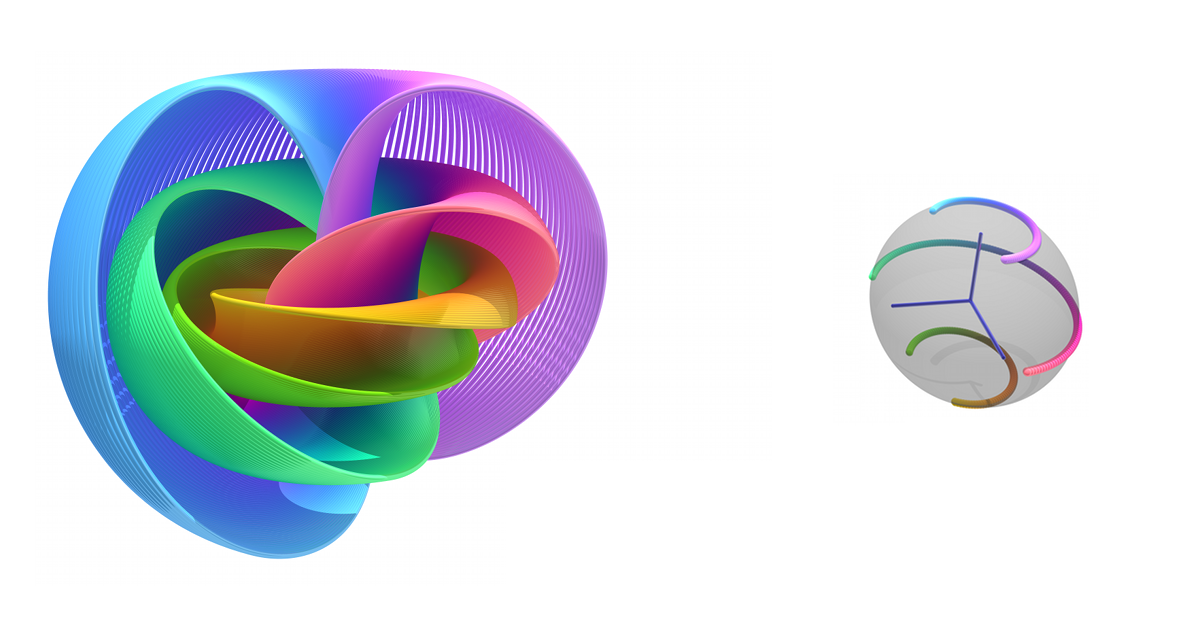
\includegraphics[width = 0.8\textwidth]{img/Hopf_Fibration.png}
\caption{Una representación de la fibración de Hopf, que lleva cada circunferencia de $\crc[3]$ a un punto en $\crc[2]$. Imagen vía \href{http://nilesjohnson.net/hopf.html}{Niles Johnson}, que tiene alguna animación chula sobre el tema.}
\label{fig:FibracionHopf}
\end{figure}

 Definimos \begin{align*}
ℂ^2 \setminus \set{0} ⊃ \set{(z,w) \tq \abs{z}^2 + \abs{w}^2 = 1 } & \longmapsto \projcp^1 \equiv \crc[2] \\
(z,w) &\longmapsto [z:w]
\end{align*}, que es una submersión, si cogemos la inversa con la norma y un montón de cuentas a las que no veo demasiado sentido.

Las fibras son circunferencias y la idea es que $f(z,w) = f(e^{iθ})(z,w))$. Pero si cogemos $\crc[2] × \crc[1]$ (o algo así) pero entonces es una submersión pero sólo localmente.

Y bueno, el grupo fundamental sí que distingue que $\crc[2] × \crc[1] \not\simeq \crc[3]$. Pero bueno, no sé qué de un discurso grandilocuente en el que nos convence que las cohomologías de De Rham son la releche y van a salvar el mundo. ¡Sálvanos, superRham!

Más cuentas. El H2 será de dimensión dos, tralarí tralará. Ok.

Por cierto, no vamos a usar estas cosas que hemos dicho hoy. Pues perfecto. Si alguien tiene ánimos que lo arregle.

\chapter{Cohomología de De Rham}
\label{chap:CohomologiaDeRham}

%% Apéndices (ejercicios, exámenes)
\appendix

\chapter{Cálculos y otras explicaciones}
% -*- root: ../GeometriaTopologia.tex -*-

Para evitarnos emborronar mucho los apuntes, ponemos en esta sección los cálculos y cuentas largas que vamos haciendo durante el curso.

\section{Proyección estereográfica de $\crc$}
\label{sec:proyeccion_estereografica_crc}

\subsection{Cálculo de las cartas}
Empecemos calculando la carta $(V_1, \alpha_1)$ con $V_1 = \crc \setminus {(0,1)}$.

Utilizando el dibujo \ref{fig:ProyEstereo} como guía, partimos de la recta $y = ax + b$. Como pasa por el polo norte, tenemos que $b = 1$, y como pasa por el punto $(s,t)$ en $\crc$, tenemos que $t=a \cdot s + 1 \implies a = \frac{t-1}{s}$; luego $y = \frac{t-1}{s} \cdot x + 1$.

Vamos a estudiar dónde se anula, ya que estamos haciendo la proyección sobre $y=0$, luego despejamos la $x$: $x = \frac{-s}{t-1} = \frac{s}{1-t}$. Y con esto ya hemos calculado la primera carta.

Ahora calculamos, de manera similar la segunda carta $(V_2, \alpha_2)$, pero esta vez proyectando desde el polo sur: partimos de la recta $y=a \cdot x+b$ y como pasa por $(s,t) \in \crc$, y en $(0,-1)$, tenemos que $y = \frac{t+1}{s} \cdot x - 1$. Proyectando sobre $y=0$, obtenemos que $x = \frac{s}{t+1}$.

\subsection{Compatibilidad de las cartas}
Veamos que son compatibles, es decir, que
\[ \appl{\alpha_2 \circ \alpha_1^{-1}}{\alpha_2(V_1 \cap V_2)}{\alpha_1(V_1 \cap V_2)} \]
está bien definida y es diferenciable.

En primer lugar, observamos que $V_1 \cap V_2 = (-\infty, 0) \cup (0, \infty)$.
En segundo lugar, para calcular la imagen de $\alpha_2 \circ \alpha_1^{-1}$, vamos a hacer la composición por pasos.

Empezamos por $x \xrightarrow{\alpha_1^{-1}} (s,t)$. Así que tenemos que calcular $(s,t)$ en función de x. Como tenemos que $x = \frac{s}{1-t}$, tomamos cuadrados $x^2 = \frac{s^2}{(1-t)^2}$, y como $(s,t) \in \crc$, tenemos que $s^2+t^2=1$.

Despejando $s^2$ y sustituyendo en $x^2$, obtenemos lo siguiente:
\[ x^2 = \frac{1 - t^2}{(1-t)^2} = \frac{(1-t)(1+t)}{(1-t)^2} = \frac{(1+t)}{(1-t)} \]

Despejamos la $t$:
\begin{gather*}
	x^2(1-t) = 1+t \iff x^2 - 1 = x^2t + t = t(x^2 + 1)\\
	t = \frac{x^2 - 1}{x^2 + 1}
\end{gather*}

Ahora nos falta despejar la s de $x = \frac{s}{1-t} \implies s = x (1-t)$. Sustituyendo la t y operando, obtenemos la expresión de $s$ en función de $x$:
\[ s = x \left(1 - \frac{x^2-1}{x^2+1}\right) = x \cdot \frac{x^2 + 1 - x^2 + 1}{x^2+1} = \frac{2x}{x^2+1} \]
Con lo que obtenemos finalmente la expresión de $(s,t)$ en función de $x$:
\[ (s,t) = \left(\frac{2x}{x^2+1}, \frac{x^2-1}{x^2+1}\right) \]

Y ahora calculamos la imagen de $(s,t)$ por $\alpha_2(s,t) = \frac{s}{1+t}$:
\[ \alpha_2\left(\frac{2x}{x^2+1},\frac{x^2-1}{x^2+1}\right) = \frac{\frac{2x}{x^2+1}}{1+\frac{x^2-1}{x^2+1}} = \dots = \frac{1}{x} \]

Luego
\[ \alpha_2 \circ \alpha_1^{-1}(x,y) = \frac{1}{x} \]


\chapter{Ejercicios}
% -*- root: ../GeometriaTopologia.tex -*-
\section{Hoja 1}

\begin{problem}[1] Considérese en $S^1$ las 2 cartas siguientes:

\[
U_1 = S^1 \setminus {(1,0)} \; \appl{φ_1^{-1}}{U_1}{(0,2π)} \text{ con } φ_1^{-1}(θ) = (\cos θ,\sin θ)
\]
\[
U_2 = S^1 \setminus {(-1,0)} \; \appl{φ_2^{-1}}{U_2}{(-π,π)} \text{ con } φ_2^{-1}(θ) = (\cos θ,\sin θ)
\]

\ppart Comprobar que estas 2 cartas definen un atlas en $S^1$.

\ppart Comprobar que el atlas anteriror es equivalente a los atlas definidos mediante la proyección estereográfica y la proyección a los ejes respectivamente.

\solution

\doneby{Dejuan}

\spart ¿$\{φ_1,φ_2\}$ es un atlas de $S^1$ si $\img(φ_1) \cup \img(φ_2) = S^1$? En caso de ser así, sólo hay que escribir las cosas con cuidado.

\spart 2 atlas son equivalentes si sus cartas son compatibles. Vamos a tomar $\{\Psi_i\}$ las cartas de las proyección estereográfica. La condición de compatibilidad es si $φ_1 \circ \Psi_1^{-1}$ es diferenciable.

Para más información, este ejercicio está esbozado ejemplificando la \ref{def::atlas_compatibles}

\end{problem}


\begin{problem}[5] Demostrar que son compactas las variedades

\ppart $\quot{ℝ^2}{ℤ^2}$

\ppart  $\projp^n$

\ppart $\projcp^n$


\solution

\doneby{Dejuan}
\spart
La relación de equivalencia que usamos para construir el espacio cociente nos dice que dos puntos $x,y ∈ ℝ^2$ pertenecen a la misma clase si existe un difeomorfismo $g ∈ ℤ^2$ tal que $g(x) = y$.
Es decir, si tenemos un par $(m,n) ∈ ℤ^2$ tal que $(x_1 + m, x_2 + n) = (y_1, y_2)$, entonces $x = (x_1, x_2)$ y $y=(y_1, y_2)$ están relacionados.

Con esta construcción, vemos que nuestro conjunto de clases de equivalencia son los puntos en $[0,1] × [0,1]$, con los bordes ``unidos'', el de arriba con el de abajo y el de la izquierda con el de la derecha. Tomando para $0<a<1$, el punto $(0,a) ~ (1,a)$, tomando $(n,m) = (1,0)$. \footnote{topológicamente estamos ante un toro (ver \fref{fig:ToroEspacioCociente})}

Esta variedad es compacta porque es ¿homeomorfa? al cuadrado $[0,1]×[0,1]\subset ℝ^2$, que es cerrado y acotado.

\spart $\projp^n$ podemos escribirlo como $\quot{\crc[n]}{\gen{J}}$, tomando y siendo $J(x_1,...,x_n) = (-x_1,...,-x_n)$.

\[\projp^n \simeq \quot{\crc[n]}{\gen{J}} \subset \real^n\]

Tenemos un conjunto cerrado y acotado en $\real^n$, con lo que es compacto.


\spart $\projcp^n = \quot{ℂ^{n+1}\setminus 0}{~}$ donde $\gx ~ \gy \dimplies ∃λ∈ℂ^{n+1} λ\gx = \gy$.

De esta manera, $\projcp^n \simeq \projp^{2n} \simeq \quot{\crc[2n]}{\gen{J}}$.

Tenemos un conjunto cerrado y acotado en $\real^{2n}$, con lo que es compacto.
\end{problem}

\begin{problem}[6]
Probar que si una variedad $M$ posee un atlas que consiste de dos cartas cuya intersección es conexa entonces $M$ es orientable. Deducir que $\crc[n]$ es orientable.

\solution

Según la \fref{def:VariedadOrientable}, una variedad es orientable si existe un atlas $A = \set{(U_i,φ_i)}_{i∈I}$ tal que $\abs{\Dif (φ_j○\inv{φ_i})} > 0$ para cualesquiera $j,i ∈ I$. Más generalmente, nos vale con que la diferencial de los difeomorfismos de cambio de carta tengan el mismo signo.

Por ser el cambio de carta un difeomorfismo, su diferencial es continua y además no se anula nunca. La única forma de que cambiase de signo es que la intersección de cartas no fuese conexa (podría saltar de valor entre componentes conexas), pero por hipótesis la intersección es conexa, luego la diferencial mantiene signo y por lo tanto la variedad es orientable.

En $\crc[n]$ se puede dar siempre un atlas con dos cartas con intersección conexa a través de la proyección estereográfica, luego es orientable.

\end{problem}

\begin{problem}[7]
Consideremos en $\real\times(-a,a)$ la acción de $ℤ$ definida por:

\[n\circ (x,λ) = (x+n,(-1)^nλ)\]

Ya hemos visto en clase que el cociente $M = \quot{ℝ×(-a,a)}{ℤ}$ es la banda de Möbius, que no es orientable.

\ppart ¿Qué variedad es el $\gor{M} = \quot{ℝ×(-a,a)}{2ℤ}$?

\ppart Demostrar que $\gor{M}$ es un cubrimiento doble de $M$ (Es decir, encontrar una aplicación diferenciable y suprayectiva $\gor{M}\to M$ tal que cada punto tiene 2 preimágenes).

\solution

\doneby{Dejuan}

Si no estamos convencidos de que el cociente $M$ sea la banda, consultar \ref{Mobius}.

No tengo muy claro si $2ℤ = \{ 2n : n∈ℤ\}$ o $2ℤ = \{0,1\}$. He tomado la primera oción.

\spart $\gor{M} = \quot{ℝ×(-a,a)}{2ℤ}$ es el cociente dado por la relación:

\[
(x,λ) ∈ ℝ×(-a,a) \sim (x',λ') \dimplies \left\{\begin{array}{cc} x' = x+n & n∈2ℤ\\λ' = (-1)^nλ & n∈2ℤ \end{array}\right.
\]

Lo primero de lo que nos damos cuenta es que $(-1)^n = 1, ∀n∈2ℤ$.

Vamos a estudiar ahora la primera componente. Vemos que $[x]∈[0,2)$, ya que $2 \sim 0$.

Con estos 2 detalles, tiene pinta de que $\gor{M}$ es el cuadrado $[-a,a]×[0,2]$ con los bordes identificados en el mismo sentido. Es decir:

\begin{figure}[hbtp]
\centering
\begin{tikzpicture}
\fill[blue!20!white] (0, -0.8) rectangle (2, 0.8);
\draw (-1.4,0) -- (3,0);
\draw (0,-1.4) -- (0,1.4);s

\node[hnlin, label = {left:$a$}] at (0, 0.8) {};
\node[hnlin, label = {left:$-a$}] at (0, -0.8) {};
\node[hnlin, label = {below right:$(2,0)$}] at (2,0) {};

\draw[blue, thick, directed]  (2, 0.8) --  (2, -0.8);
\draw[blue, thick, directed] (0, 0.8) -- (0,-0.8);
\end{tikzpicture}
\end{figure}

Estamos ante un cilindro de altura $2a$ sin tapas.\footnote{Normalmente, los cilindros sin tapa se llaman tubos.}


\spart

Buscamos $g$ tal que $∀(x',λ') ∈\gor{M}, ∃(x_1,λ_1),(x_2,λ_2)∈M$ con $(x_1,λ_1)≠(x_2,λ_2)$ y que se cumpla $g(x_1,λ_1) = g(x_2,λ_2) = (x',λ')$

Tomando la proyección de $\gor{M}$ en $M$, tenemos una aplicación diferenciable (por ser identidades o cambios de signo o desplazamiento) en el que cada punto de $M$ tiene 2 preimágenes:

\[
	\left.
		\begin{array}{c}
			(x,λ) ∈ M \\
			(x',λ) ∈ \gor{M}\\
			(x+1',-λ) ∈ \gor{M}
		\end{array}
	\right\}
	\to π^{-1}(x'+1,(-1)^1(-λ)) = π^{-1}(x',(-1)^0λ) = (x,λ)
\]

\begin{figure}[hbtp]
\centering
\begin{tikzpicture}
\fill[pattern=north east lines, pattern color=blue!70!white] (0, -0.8) rectangle (2, 0.8);
\fill[pattern=north west lines, pattern color=red!50!white]  (0, -0.8) rectangle (1, 0.8);

\draw (-1.4,0) -- (3,0);
\draw (0,-1.4) -- (0,1.4);

\node[hnlin, label = {left:$a$}] at (0, 0.8) {};
\node[hnlin, label = {left:$-a$}] at (0, -0.8) {};
\node[hnlin, label = {below right:$(2,0)$}] at (2,0) {};

\draw[blue, thick, directed]	(2, 0.8) --  (2, -0.8);
\draw[blue!50!red, thick, directed]	(0, 0.8) -- (0,-0.8);
\draw[red,	thick, directed]	(1,-0.8) -- (1,0.8);

\node[label = {left:$3$}] at (1.8, 0.5) {};
\node[label = {left:$2$}] at (1.8, -0.5) {};
\node[label = {left:$1$}] at (0.8, -0.5) {};
\node[label = {left:$4$}] at (0.8, 0.5) {};

\end{tikzpicture}
\caption{En rojo la variedad $M$ y en azul, $\gor{M}$}
\label{ej:1.7}
\end{figure}

Con la aplicación $π$ descrita anteriormente y representada en \fref{ej:1.7}, vemos que se corresponden los cuadrantes $1,3$ de $\gor{M}$ con el cuadrante $1$ de $M$ y los cuadrantes $2,4$ de $\gor{M}$ con el cuadrante $2$ de $M$. De esta manera, todo punto de $M$ tiene 2 preimágenes en $\gor{M}$.


\end{problem}

\begin{problem}[8] Sean $M$ y $N$ dos variedades orientables, y sea $\appl{f}{M}{N}$ una aplicación diferenciable.

\ppart Define el concepto de morfismo que preserva la orientación y pon un ejemplo de uno (y de otro que no lo sea).

\ppart Demostrar que una variedad cociente $\quot{M}{G}$ en la que $M$ es orientable y los elementos de $G$ preservan la orientación es orientable.

\ppart Deducir que los espacios proyectivos de dimensión impar son orientables.

\solution

\spart

La definición de orientación de Geometría Diferencial \citep[Def. IV.7]{ApuntesGeoDif} era bastante cómoda, ya que sólo dependía de la existencia de una $n$-forma de volumen que no se anulase. La cuestión es que dudo bastante que podamos usar eso aquí, así que toca ir a la definición fea, dependiente de las cartas.

\begin{defn}[Aplicación\IS compatible con la orientación] Sean $M$ y $N$ dos variedades orientables, y sea $\appl{f}{M}{N}$ una aplicación diferenciable. Diremos que $f$ es compatible con la orientación (o que preserva la orientación) si y sólo si, para dos cartas cualesquiera $(U_i, φ_i)$ y $(U_j, φ_j)$ de $M$ y $N$ respectivamente, el jacobiano dado por \[ \Dif (φ_i ○ f ○ \inv{φ_j})\] es positivo en la región en la que esté definido.
\end{defn}

Los ejemplos no se me ocurren ahora.

\spart

\end{problem}

\section{Hoja 2}

\begin{problem}[1]

Demostrar que $\crc[3]$ es un grupo de Lie.

\solution

$\crc[3]$ es un grupo de Lie si admite una estructura de grupo. $\vec{u} \in \crc[3] \implies \vec{u} = a + bi + cj + dk, \norm{\vec{u}} = 1$, siendo $i,j,k$ las raíces cuartas de la unidad.

Tenemos que comprobar que

\[\vec{x},\vec{y}\in\crc[3] \implies \vec{x}·\vec{y} \in\crc[3]\]

Para ello comprobamos:

\[
(a+bi+cj+dk)(a'+b'i+c'j+d'k) = ... = 1 \to \norm{\vec{x}·\vec{y}} = 1
\]
\end{problem}

\begin{problem}[2]
¿Qué variedad es $M^2\#\crc[2]$? ¿Y en general $M^n\#\crc[n]$?
\solution

\[M^n\#\crc[n] = M^n\]

Porque al sumar conexamente con esferas, obtenemos variedades homeomorfas.

\end{problem}

\begin{problem}[3]

\ppart Demostrar que un abierto de una variedad orientable es él mismo una variedad orientable.

\ppart Deducir de ahí que $\projp^n$ y la superficie $\mathbb{K}$ de Klein son no
orientables.

\solution

\spart Supongamos que tenemos una variedad $M$ orientable que contiene un abierto $A$ que no es orientable. Si $A$ no es orientable, entonces existen cartas en un atlas tal que $|\det(φ_j\circ φ_i)| ≤ 0$.
Bastaría con incluir estas cartas compatiblemente en el atlas de $M$ para obtener que no es orientable, lo que, por hipótesis, no es cierto.

\spart Si los abiertos de variedades orientables son en sí mismos variedades orientables, ni$\projp^n$ ni $\mathbb{K}$ pueden ser variedades orientables puesto que contienen un abierto que es la cinta de Mobius.
\end{problem}

\begin{problem}[4] Exhibir una triangulación del toro $\torus = \crc[1] × \crc[1] = \quot{ℝ^2}{ℤ^2}$ que pruebe que $χ(\torus) = 0$.

\solution

Consultar la \fref{fig:TriangulacionToroPlano}.

Para ver que $\chi(\mathbb{T}_2) = 0$, contamos en la triangulación:

\[V-A+C = 9 - 27 + 18 = 0\]

\end{problem}

\begin{problem}[5]
Demostrar
\[\chi(M_1\#M_2) = \chi(M_1) + \chi(M_2) - 2\]

Deducir $\chi(M^2)$ para cualquier superficie orientable.

\solution

La unión de la suma conexa superpone 2 circunferencias, que podríamos tomar como homeomorfas a un triángulo, con lo que estamos quitando un triángulo.

La $\chi(M_1\#M_2) = \chi(M_1) + \chi(M_2) - cosas$, donde esas cosas que hay que quitar son 3 vértices repetidos (los 3 del triángulo), 3 aristas y 2 caras (una de cada variedad), es decir:

\[\chi(M_1\#M_2) = \chi(M_1) + \chi(M_2) - (3-3+2) = \chi(M_1) + \chi(M_2) - 2\]

Cualquier superficie orientable $M^2$ es, según el \fref{thm:ClasificacionSuperficies}, una suma conexa de toros. Dado que la característica del toro es $0$, las superficies orientables tendrán característica par negativa.
\end{problem}

\begin{problem}[6] Demostrar que $\chi(\projp^2) = 1$ y deducir $\chi(M^2)$ para cualquier superficie no orientable.

\solution

De nuevo según el \fref{thm:ClasificacionSuperficies}, cualquier superficie compacta no orientable es una suma de planos proyectivos, luego su característica será también negativa.

\end{problem}

\section{Hoja 3}

\begin{problem}[6]

\ppart Comprobar que si $M$ y $N$ son dos variedades la proyección obvia $M × N \mapsto N$ es una submersión.

\ppart Comprobar que la fibración de Hopf es una submersión. ¿Cuáles son sus fibras?

\solution

\spart

Según la \fref{def:Submersion}, simplemente tenemos que ver que la proyección es sobreyectiva (obvio) y que su diferencial es sobreyectiva, esto es, que tiene rango máximo (que también tiene, ya que es la identidad).

\spart

Ver \fref{sec:FibracionHopf}.

\end{problem}

\section{Hoja 4}

\begin{problem}[4] Se considera la forma diferencial $ω = x \dif y - y \dif x ∈ Ω(ℝ^2)$. Demostrar que si $\appl{i}{\crc[1]}{ℝ^2}$ denota la aplicación inclusión entonces $i^*(ω) = \dif θ$. Habrá que ver que $i^*ω (∂θ) = 1$.

\solution

\doneby{Guille}

La aplicación inclusión vendrá dada por \[ i(θ) = (\cos θ, \sin θ) \], y entonces \[ i^*ω = \cos θ · (\cos θ \dif θ) - \sin θ (- \sin θ \dif θ) = \dif θ \]

\end{problem}


\begin{problem} Se consideran las formas diferenciales $ω = \sin x \dif y ∧ \dif z$ y $η = \cos x \dif t$, ambas en $Ω(ℝ^4)$. Calcular:

\ppart $\dif ω,\,\difη,\, (ω∧η),\, \dif(ω∧η), \, \difω ∧ η$

\ppart $\dif \dif ω,\, \dif \dif η, \, \dif \dif (ω ∧ η)$.

\ppart $f^*\dif ω, \dif f^* ω$, donde $f(x,y,z,t) = (y, x^2, z + t, t-z)$

\ppart $f^*(ω∧η),\, f^*ω ∧ f^*η$ donde $f$ es la aplicación del apartado anterior.

\solution

\spart

\begin{gather*}
\dif ω = \cos x \dif x ∧ \dif y ∧ \dif z \\
\dif η = - \sin x \dif x ∧ \dif t \\
ω ∧ η = \sin x \cos x \dif y ∧ \dif z ∧ \dif t \\
\dif(ω∧η) = (\cos^2 x - \sin^2 x) \dif x ∧ \dif y ∧ \dif z ∧ \dif t \\
\dif ω ∧ η = 0 \\
ω ∧ \dif η = 0
\end{gather*}

\spart

Todas cero por ser diferenciales de diferenciales.

\spart

\begin{gather*}
f^* \dif ω = \cos y · (\dif y) ∧ (2x \dif x) ∧ (\dif z + \dif t) \\
f^* ω = \sin y (2x \dif x ) ∧ (\dif z + \dif t) \\
\dif f^* ω = \cos y ·2x \dif y ∧ \dif x ∧ (\dif z + \dif t) \\
f^* \dif η = - \sin y (\dif y) ∧ (\dif t - \dif z) \\
f^* η = \cos y (\dif t - \dif z) \\
\dif f^* η = -\sin y \dif y ∧ (\dif t - \dif z)
\end{gather*}

\spart

\begin{align*}
f^*(ω∧η) &= \sin y \cos y (2x \dif x) ∧ (\dif z + \dif t) ∧ (\dif t - \dif z) = \\
	&=2x \sin y \cos y \dif x ∧ \dif z ∧ \dif t - 2x \sin y \cos y \dif x ∧ \dif t ∧ \dif z = \\
	&= 4x \sin y \cos y \dif x ∧ \dif z ∧ \dif t \\
f^*ω ∧ f^* η &= \left(\sin y (2x \dif x ) ∧ (\dif z + \dif t)\right) ∧ \left(\cos y (\dif t - \dif z)\right ) = \\
	&= 4x \sin y \cos y \dif x ∧ \dif z ∧ \dif t
\end{align*}

\end{problem}

\section{Hoja 5}

\begin{problem}[1]
Sea $\appl{f}{M}{N}$ una aplicación diferenciable. Probar que $\appl{f^\ast}{H^\ast(N)}{H^\ast(M)}$ es un homomorfismo de anillos y que si f es un difeomorfismo este homorfismo es un isomorfismo.
\solution

$f^\ast$ es un homomorfismo de anillos porque $f^\ast(a+ b) = f^\ast(a) + f^\ast(b)$ y $f^\ast(a\wedge b) = f^\ast(a) \wedge f^\ast(b)$ (ambas igualdades por definición de pullback).

Si $f$ fuera difeomorfismo, podemos definir $(f^\ast)^{-1}$ siendo $f^\ast$ biyectiva y continua, es decir, es un isomorfismo.
\end{problem}



\begin{problem}[3]
Demostrar que $\crc[n]$ es un retracto de deformación de $\real^{n+1} \setminus {0}$
\solution
Por la proyección estereográfica
\end{problem}

\begin{problem}[4]
 En $\real^2 \setminus {0}$ se consideran las 1-formas


\[ω1 = xdy − ydx\]

\[ω2 = \frac{xdy − ydx}{x^2+y^2}\]

Investigar si alguna de ellas genera  $H^1(\real^2 \setminus {0})$.

\solution

$H^k$ es el espacio de las k-formas cerradas que no son exactas.
%
Sabemos que tiene dimensión 1 ya que $h^1(\crc[1])=1$.
%
Además, por el ejercicio 3 y \ref{crl:CohomHomotopia}: $H^1(\crc[n]) = H^1(\real^{n+1} \setminus 0) = 1$

Si alguna de estas 1-formas fuera cerrada y no exacta, estaría en $H^1(\real^2\setminus {0})$ y sería generador ya que este e.v. tiene dimensión 1.

Vamos a verlo:

\[\dif ω_1 = 2\dif x\wedge \dif y\]

\[\dif ω_2 = ... = 0\]

$ω_2$ es cerrada.
%
Para ver si es exacta, tomamos $\appl{i}{\theta}{(\cos θ,\sin θ)}$ y hacemos:

\[
i^\ast ω_2 = ... = \dif θ
\]

Entonces tendríamos que $ω$ es exacta, porque tomamos: $θ = i^\ast µ$ para alguna $µ$ que debería existir (espero) y diferenciando:

\[
i^\ast ω_2 = \dif θ = \dif (i^\ast µ) = i^\ast(\dif µ)
\]

Como ninguna de las dos es cerrada y no exacta, no están en $H^1(\real^2\setminus{0})$ luego no pueden generarlo.

\end{problem}


\begin{problem}[5]

Dada una sucesión exacta \[ 0 \to V_0 \xrightarrow{h_0} V_1 \to \dotsb \to V_{n-1} \xrightarrow{h_{n-1}} V_{n} \to 0 \] Demostrar que la suma alternada de dimensiones de los espacios vectoriales es cero, es decir:  \[ \sum_{i=0}^n (-1)^i \dim V_i = 0\]


\solution

Consultar \fref{prop:sumaAlternada0}

\end{problem}

\begin{problem}[6]
Sea M una variedad compacta. Construir una partición de la unidad de M subordinada al cubrimiento por abiertos de M que se definió en clase.
\solution
Consultar \fref{thm:SucesionMayerVietoris}
\end{problem}

\begin{problem}[7]

\ppart Calcular los grupos de cohomología de $\crc[n]$ razonando por inducción a partir de los de $\crc[1]$.
\ppart Deducir que si $n ≠ m$ entonces $ℝ^n$ no es homeomorfo a $ℝ^m$.
\ppart Deducir también el Teorema del punto fijo de Brower.

\solution

\spart
\label{ej:Hoja7:CohomologiaSN}

En \eqref{eq:CohomologiaS1} y \eqref{eq:CohomologiaS2} veíamos la cohomología de $\crc[1]$ y $\crc[2]$ respectivamente, así que la base de inducción ya la tenemos. Vamos ahora a por el resto, y lo haremos aplicando Mayer-Vietoris con los siguientes abiertos:
\begin{align*}
U &= \crc[n] \setminus \set{N} \\
V &= \crc[n] \setminus \set{S}
\end{align*} donde $N, S$ son dos puntos distintos de la circunferencia (no hace falta que sean antipodales. Esto nos da la intersección $U ∩ V \simeq \crc[n-1]$.

Construimos la cadena de Mayer-Vietoris (\fref{fig:MayerVietorisSN}), de donde sacamos rápidamente que $h^1(\crc[n]) = 0$ (tenemos $1 - 2 + 1 + h^1(\crc[n]) = 0$), que $h^k(\crc[n]) = 0$ cuando $1 < k < n$ (la cadena es exacta con sólo $H^k(\crc[n])$) en el medio y, para el último caso, que $h^n(\crc[n]) = 1$, que es efectivamente lo que teníamos que sacar \eqref{eq:CohomologiaSN}.

\begin{figure}[hbtp]
\centering
\tikzexternaldisable
\begin{tikzcd}[row sep = 15pt]
0 \rar
	& \overbracket{H^0(\crc[n])}^{\dim 1} \rar
	& \overbracket{H^0(U) \oplus H^0(V)}^{\dim 2} \rar
	& \overbracket{H^0(U ∩ V)}^{\dim 1} \arrow[snake]{dll}{}
	\\
	& H^1(\crc[n]) \rar
	& \overbracket{H^1(U) \oplus H^1(V)}^{\dim 0} \rar
	& \overbracket{H^1(U ∩ V)}^{\dim 0} \arrow[snake]{dll}{}
	\\
	& H^2(\crc[n]) \rar
	& \overbracket{H^2(U) \oplus H^2(V)}^{\dim 0} \rar
	& \overbracket{H^2(U ∩ V)}^{\dim 0} \arrow[snake]{dll}{}
	\\
	& \phantom{H^1(\crc[n])}
	& \dotsb
	& \phantom{H^1(U ∩ V)} \arrow[snake]{dll}{}
	\\
	& H^{n-1}(\crc[n]) \rar
	& \overbracket{H^{n-1}(U) \oplus H^{n-1}(V)}^{\dim 0} \rar
	& \overbracket{H^{n-1}(U ∩ V)}^{\dim 1} \arrow[snake]{dll}{}
	\\
	& H^{n}(\crc[n]) \rar
	& \overbracket{H^{n}(U) \oplus H^{n}(V)}^{\dim 0} \rar
	& H^{n}(U ∩ V) \rar & 0 \\
\end{tikzcd}
\tikzexternalenable
\caption{Cadena de Mayer-Vietoris para $\crc[n]$, tomando $U = \crc[n] \setminus \set{N}$, $V = \crc[n] \setminus \set{S}$ y $U ∩ V = \crc[n-1]$.}
\label{fig:MayerVietorisSN}
\end{figure}

\spart

Podemos quitarle un punto cualquiera a ambos y ver que salen dos cosas que no son homeomorfas ($ℝ^n \setminus \set{p} \simeq \crc[n] \not\cong \crc[m] \simeq ℝ^m \setminus \set{q}$).

\doneby{Dejuan} $h^n(\real^n) = 1 ≠ h^n(\real^m) \to \real^n\not\cong \real^m$ 

\spart

Vamos a ver qué nos dice el teorema.

\begin{theorem}[Teorema\IS del punto fijo de Brouwer] \label{thm:PuntoFijoBrower} Sea $\appl{f}{\disc}{\disc}$ una aplicación continua. del disco cerrado en $ℝ^n$ en sí mismo. Entonces $f$ tiene un punto fijo.
\end{theorem}

\end{problem}


\begin{problem}[9]

\ppart Calcular los grupos de cohomología de $\real^2$ menos n puntos.
\ppart Y la de $\real^3$ menos un punto y una recta.
\ppart Y la de un toro menos un punto.

\solution
\doneby{Dejuan}

No tengo ni idea de calcular los grupos de cohomologías, asique me contentaré con calcular las dimensiones. 
%
Aunque supongo que la única posibilidad de dimensión 1 es $\real$, ya que $H^n(\real^n) = \real$ con $h^1(\real^n) = 1$.

\spart 
Tomamos $n=2$ para ejemplificar.
%
$U = \real^2\setminus\{p_1\}$ y $V=\real^2\setminus\{p_2\}$ de tal manera que $U\cap V = \real^2\setminus \{p_1,p_2\}$

\[
	\underbrace{h^0(\real^2)}_{1} \to 
	\underbrace{h^0(U)\oplus h^0(V)}_{1+1=2} \to 
	\underbrace{h^0(U\cap V)}_{1} \to 
	\underbrace{h^1(\real^2)}_{0} \to 
	\underbrace{h^1(U)\oplus h^1(V)}_{1+1=2} \to 
	\underbrace{h^1(U\cap V)}_{x} \to 
	\underbrace{h^2 (\real^2)}_{0}
\]
Por la suma alternada, $0-2+x-0=0 \to x=2$.


Tomamos $n=3$:
%
$U = \real^2\setminus\{p_1,p_2\}$ y $V=\real^2\setminus\{p_3\}$ de tal manera que $U\cap V = \real^2\setminus \{p_1,p_2,p_3\}$

\[
	\underbrace{h^0(\real^2)}_{1} \to 
	\underbrace{h^0(U)\oplus h^0(V)}_{1+1=2} \to 
	\underbrace{h^0(U\cap V)}_{1} \to 
	\underbrace{h^1(\real^2)}_{0} \to 
	\underbrace{h^1(U)\oplus h^1(V)}_{2+1=3} \to 
	\underbrace{h^1(U\cap V)}_{x} \to 
	\underbrace{h^2 (\real^2)}_{0}
\]

Por la suma alternada, $0-3+x-0=0 \to x=3$.

Por inducción, podemos probar que $h^1(\real^2 \setminus\{p_1,...,p_n\}) = n$ (tomando $h^0(\real^2 \setminus\{p_1,...,p_n\})$ por número de componentes conexas).

\spart Suponemos que el punto no pertenece a la recta.
%
Como son 2 componentes conexas, podemos trabajar por separado.


\end{problem}


\section{Hoja 6}

\begin{problem} Sean $\appl{π_1, π_2}{M × N}{M,N}$ las dos proyecciones obias. Probar que si $ω$ y η son dos formas cerradas en $M$ y $N$ respectivamente (y por tanto definen clases de cohomología en $M$ y $N$) entonces $π_1^* ω ∧ π_2^* η$ es una forma cerrada de $M × N$ y por tanto define una clase de cohomología en $M × N$.

\solution

\doneby{Guille}

Simplemente usando las propiedades de la diferencial (\fref{prop:PropsDiferencial}) sale: \begin{align*}
\dif (π_1^* ω ∧ π_2^* η)
	&= \dif π_1^* ω ∧ π_2^* η + (-1)^{\deg π_1^* ω} π_1^* ω ∧ \dif π_2^* η = \\
	&= π_1^*(\dif ω ) ∧ π_2^* η + (-1)^{\deg π_1^* ω} π_1^* ω ∧ π_2^* (\dif η) = \\
	&= 0 + 0 = 0
\end{align*}

\end{problem}

\begin{problem} Calcular la cohomología de las siguientes variedades:

\ppart $\torus = \crc[1] × \crc[1]$.
\ppart $\crc[n] × \crc[m]$.
\ppart $\crc[3] × T_g$.
\ppart $\crc[1] × \crc[1] × \crc[1]$.

\solution

\doneby{Guille}

\spart

Ya esta hecho en la \fref{sec:CaracteristicaEulerPoincare} usando el \nref{thm:Kunneth} (salen grupos de dimensión 1, 2, 1 en ese orden).

\spart

Aplicamos de nuevo el \nref{thm:Kunneth}, y basándome en la cohomología de $\crc[n]$ \eqref{eq:CohomologiaSN} me voy a tirar el siguiente triple: \[ h^k(\crc[n] × \crc[m]) = \begin{cases}
1 & k = 0 \\
1 & k = n, m \\
1 & k = n + m \\
0 & \text{otro caso}
\end{cases}\]

Si $n = m$, entonces el caso $k = n = m$ sale de dimensión 2.

\spart

No sé qué es $T_g$.

\spart

Aplicamos Mayer-Vietoris con los siguientes conjuntos: \begin{align*}
U &= \crc × \crc × (\crc \setminus p) \\
V &= \set{0} × \set{0} × \bola_ε(p)
\end{align*} considerando $\bola_ε(p)$ como un cacho de la circunferencia. Luego lo completo

\end{problem}

\begin{problem}[4] Probar que $χ(M × N) = χ(M) χ(N)$. ¿Y desde el punto de vista de triangulaciones?

\solution

\doneby{Guille}

Sabemos por una parte que la \nlref{def:CaracteristicaEulerPoincare} es \[ χ(M) = \sum_{k=0}^m (-1)^k h^k(M) \] y por el \nref{thm:Kunneth} que la dimensión de la variedad producto es \[ h^k(M × N) = \sum_{p + q = k} h^p(M) h^q(N) \] luego \[ χ(M ×N) = \sum_{k = 0}^{m + n} (-1)^k\sum_{ p + q = k} h^p(M) h^q(N) \]

Haciendo el producto por el otro lado: \[ χ(M) χ(N) = \sum_{p = 0}^m (-1)^p h^p(M) · \sum_{q = 0}^n (-1)^q h^q(N) = \sum_{p = 0}^m \sum_{q=0}^n (-1)^{p+q} h^p(M) h^q(N) \] y parece que es lo mismo.

Por triangulaciones ni idea.

\end{problem}

\begin{problem}[7] Sea $M = ℝ^2 \setminus \set{p_1, \dotsc, p_n}$ con $p_k = (a_k, b_k)$.

\ppart Probar que \[ ω_i = \frac{(x - a_i) \dif y - (y - b_i) \dif x}{(x-a_i)^2 + (y-b_i)^2} \] define un elemento no nulo de $H^1(M)$.

\ppart Probar que si los puntos $P_i$ son distintos las clases de cohomología inducidas por $n$ diferenciales anteriores son linealmente independientes.

\ppart  Demostrar que $ω = P(x,y) \dif x + Q(x,y) \dif y ∈ Ω^1(M)$ es cerrada si y sólo si el campo $F = P∂_x + Q ∂_y$ es irrotacional (i.e., satisface Green) y que es exacta si y sólo si $F$ es conservativo.

\ppart Demostrar que $F$ es un campo conservativo si y sólo si \[ \int_{γ_i} F = \int_{γ_i} ω = 0\] donde $γ_i$ es una circunferencia centrada en $p_i$ que no contiene a ningún otro $p_j$.

\solution

\doneby{Guille}

\spart

Primero vemos que $ω_i ∈ H^1(M)$, esto es, que $\dif ω_i = 0$. Eso sale rápido:
\[ \dif ω_i = \frac{\dif x ∧ \dif y - \dif y ∧ \dif x}{(x-a_i)^2 + (y-b_i)^2} = 0\]

Para ver que no es nula, tenemos que ver que no es exacta. Hagámoslo por reducción al absurdo, y supongamos que existe una $0$-forma η tal que $\dif η = ω$. En ese caso podemos aplicar el teorema de Stokes, que nos dice que $\int_{∂Ω} η = \int_Ω \dif η$. En particular, podemos tomar $Ω = \crc$ con la circunferencia centrada en $p_i$, luego $∂\crc = ∅$, así que tenemos que tener $\int_{\crc} ω = 0$ si fuese exacta. Ahora veremos que esa integral en realidad no es nula.

Para integrar, hacemos el cambio a polares, que es perfectamente válido en un entorno de $p_i$: \[ \begin{cases} x = r \cos θ + a_i \\ y = r \sin θ + b_i \end{cases} \implies
\begin{cases}
\dif x = \cos θ \dif r - r \sin θ \dif θ \\
\dif y = \sin θ \dif r + r \cos θ \dif θ \\
\end{cases}\]

Sustituyendo: \[ \tilde{ω}_i =  \frac{r \cos θ (\sin θ \dif r + r \cos θ \dif θ) - r \sin θ (\cos θ \dif r - r \sin θ \dif θ)}{(r \cos θ)^2 + (r \sin θ)^2} = \frac{r^2 \cos^2 θ \dif θ + r^2 \sin^2 θ \dif θ}{r^2} = \dif θ \]

Cuidado que aunque parezca que nos ha salido exacta en realidad no es así, principalmente porque $θ(x,y)$ no es una función que podamos definir (el cambio de coordenadas no es inyectivo en $θ$). De hecho, si hacemos la integral que decíamos antes, lo que nos va a quedar es que \[ \int_{\crc} ω_i = \int_0^{2π} \dif θ = 2π ≠ 0 \] por lo que efectivamente $ω_i$ no es exacta.

\spart

Esto no sé cómo sacarlo.

\spart

Supongo que Gabino se refiere a que $P_y = Q_x$ con lo de ``satisface Green'', lo que efectivamente da que $\dif ω = 0$. Lo de que es conservativo implica que sea el gradiente de una función (esto es, $\Dif f = F$) y efectivamente da que es exacta.

\spart

\end{problem}


\bibliography{../Apuntes}{}
\printindex
\end{document}
